%==============================================================================
% queues-performance.tex
%==============================================================================

\chapter{Performance}
\label{chap:queues-performance}

We evaluate the performance of the different queue implementations
when used by the intervals scheduler with a variety of parallel Java
Grande Forum benchmarks (Appendix \ref{chap:appendix-benchmarks}) on
two different machines:

\begin{itemize}
\item Intel Core2 Duo with one processor and two cores, running Ubuntu
  10.04 64-bit with kernel 2.6.32 and Sun Hotspot JDK 1.6.0\_20
  (Appendix \ref{sec:experimental-setup-marvin})
\item Intel Nehalem with two processors and eight cores, running
  Ubuntu 9.04 64-bit with kernel 2.6.29 and Sun Hotspot JDK 1.6.0\_20
  (Appendix \ref{sec:experimental-setup-mafushi})
\end{itemize}

Both machines invoke the JVM with the following parameters:

\begin{lstlisting}
  -server -Xmx2048M -Xms2048M -Xss8m
\end{lstlisting}

The execution time reported is the average of the three best benchmark
iterations from ten separate invocations.


\section{Intervals}
\label{sec:queues-performance-intervals}

The performance of the intervals implementation of the JGF benchmarks
is comparable to the threaded implementation (Figure
\ref{fig:queues-performance-threads}).

\begin{figure}[htb]
  \centering
  \subfloat[Intel Core2 Duo: 2 threads, 2 workers]{
    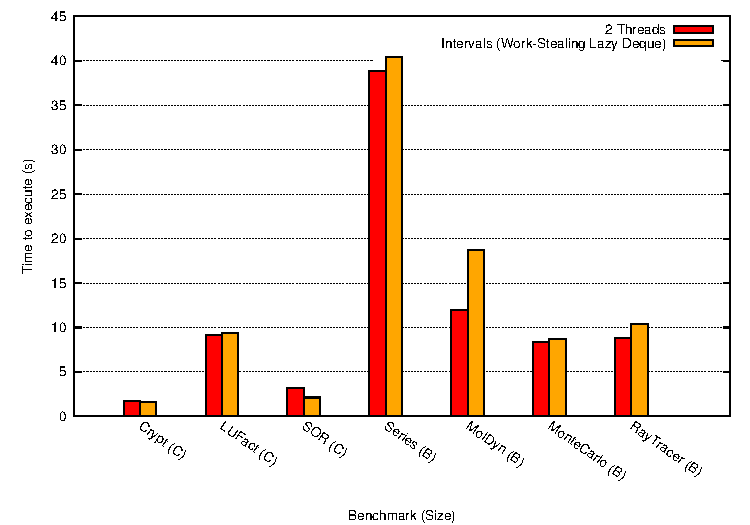
\includegraphics[width=0.5\linewidth]{queues-performance/marvin-threads}
    \label{fig:queues-performance-marvin-threads}
  }
  \subfloat[Intel Nehalem: 8 threads, 8 workers]{
    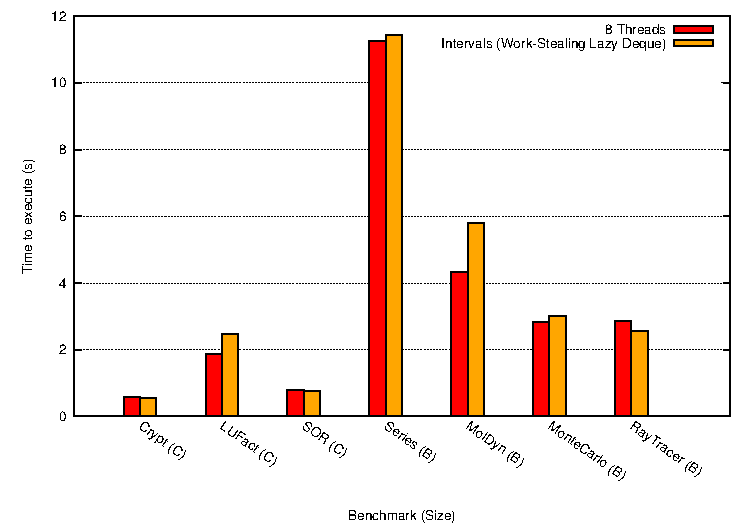
\includegraphics[width=0.5\linewidth]{queues-performance/mafushi-threads}
    \label{fig:queues-performance-mafushi-threads}
  }
  \caption{Threads and intervals benchmarks running on Intel Core2 Duo
    (Appendix \ref{sec:experimental-setup-marvin}) and Intel
    Nehalem (Appendix \ref{sec:experimental-setup-mafushi})}
  \label{fig:queues-performance-threads}
\end{figure}

The only benchmarks where intervals are considerably slower than
threads \emph{LuFact} and \emph{MolDyn}. The main reason is that the
way work is distributed between intervals makes the workers run out of
work too often. When a worker runs out of work, it becomes idle and
only wakes up if a new work item is added to its queue. Idle workers
acquire a local semaphore which blocks until release is invoked by
some other worker and are added to a global idle list guarded by a
shared lock. If there is an idle worker, adding a new work item
releases the semaphore of the worker and removes it from the idle
list.

Putting a worker to sleep and waking up again is quite
expensive. Compared to other benchmarks, workers in \emph{LuFact} and
\emph{MolDyn} run out of work more often (Table
\ref{tab:queues-performance-threads}).

\begin{table}[htb]
  \centering
  \subfloat[Intel Core2 Duo]{
    \begin{tabular}{|l*{5}{|c}|}
      \hline
      & \emph{LuFact} (C) & \emph{MolDyn} (B) & \emph{Crypt} (C) & \emph{SOR} (C) & \emph{RayTracer} (B) \\
      \hline
      Idle & 3533 & 271 & 9 & 6 & 6 \\
      Woke up & 3531 & 269 & 7 & 4 & 4 \\
      \hline
    \end{tabular}
    \label{tab:queues-performance-marvin-threads}
  }
  \\
  \subfloat[Intel Nehalem]{
    \begin{tabular}{|l*{5}{|c}|}
      \hline
      & \emph{LuFact} (C) & \emph{MolDyn} (B) & \emph{Crypt} (C) & \emph{SOR} (C) & \emph{RayTracer} (B) \\
      \hline
      Idle & 11226 & 1057 & 27 & 22 & 17 \\
      Woke up & 11218 & 1051 & 19 & 14 & 9 \\
      \hline
    \end{tabular}
    \label{tab:queues-performance-mafushi-threads}
  }
  \caption[Idle workers]{Times workers run out of work and become idle, and get woken up again}
  \label{tab:queues-performance-threads}
\end{table}


\section{Work-Stealing Queues}
\label{sec:queues-performance-ws}

When comparing our implementations of the work-stealing queue,
\emph{Work-Stealing Deque} (Section
\ref{sec:queues-implementation-ws-deque}) and \emph{Idempotent
  Work-Stealing Deque} (Section
\ref{sec:queues-implementation-idempotent-ws-deque}), with the
original \emph{Work-Stealing Lazy Deque} (Section
\ref{sec:queues-background-current-implementation}) we do not see a
significant difference in the runtime of the JGF benchmarks (Figure
\ref{fig:queues-performance-deques}) on both machines we tested them
on.

\begin{figure}[!ht]
  \centering
  \subfloat[Intel Core2 Duo]{
    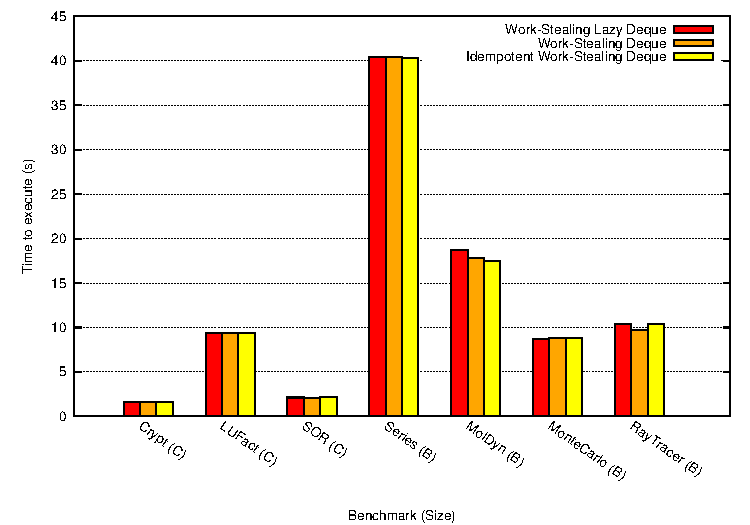
\includegraphics[width=0.68\linewidth]{queues-performance/marvin-deques}
    \label{fig:queues-performance-marvin-deques}
  }
  \\
  \subfloat[Intel Nehalem]{
    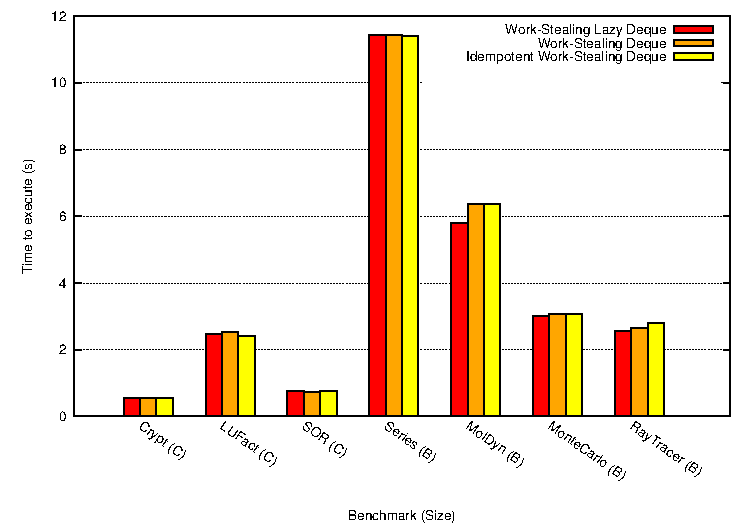
\includegraphics[width=0.68\linewidth]{queues-performance/mafushi-deques}
    \label{fig:queues-performance-mafushi-deques}
  }
  \caption{Deques benchmarks running on Intel Core2 Duo (Appendix
    \ref{sec:experimental-setup-marvin}) and Intel Nehalem (Appendix
    \ref{sec:experimental-setup-mafushi})}
  \label{fig:queues-performance-deques}
\end{figure}

The \emph{Work-Stealing Lazy Deque} implementation is very efficient
already. Using a lock in the \lstinline!steal()! method is of less
impact than we thought it would be.

\emph{Work-Stealing Lazy Deque} uses an
\lstinline!AtomicReferenceArray! to maintain work items. The
\lstinline!AtomicReferenceArray! provides volatile access semantics
for its array elements, which is not supported for ordinary
arrays. Because of this, \emph{Work-Stealing Lazy Deque} does not have
to use additional volatile or atomic variables like the other deque
implementations do. This allows for a simpler implementation.

The owner of the deque \emph{Work-Stealing Lazy Deque} only lazily
updates the location of the deque's head. This means it only updates
the head when its owner tries to take a work item and finds it was
stolen by a competing thief. As opposed to the methods
\lstinline!take()! and \lstinline!steal()!  of the \emph{Work-Stealing
  Deque} which attempt to update the location of the deque's head on
every execution with a Compare-and-Swap operation. Similarly the
methods \lstinline!take()! and \lstinline!steal()! of the
\emph{Idempotent Work-Stealing Deque} have to update the size of the
deque in the anchor on every execution.

Another reason for the lack of difference between the queue
implementations might be the small number of cores of the systems we
had to test them on (see Section
\ref{sec:queues-performance-shared-queue} for more details).


\section{Alternative Work-Stealing Queues}
\label{sec:queues-performance-alternative}

\subsection{Dynamic Work-Stealing Deque}
\label{sec:queues-performance-alternative-dynamic}

The implementation of the \emph{Dynamic Work-Stealing Deque} (Section
\ref{sec:queues-alternative-implementations-dynamic-deque}) requires
extra work for the list's maintenance which reflects in its
performance (Figure \ref{fig:queues-performance-dynamic}).

\begin{figure}[!htb]
  \centering
  \subfloat[Intel Core2 Duo: 2 threads, 2 workers]{
    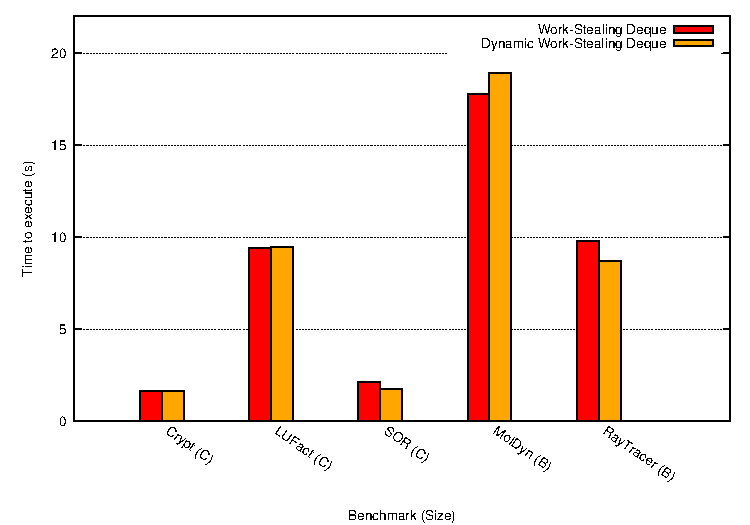
\includegraphics[width=0.5\linewidth]{queues-performance/marvin-dynamic}
    \label{fig:queues-performance-marvin-dynamic}
  }
  \subfloat[Intel Nehalem: 8 threads, 8 workers]{
    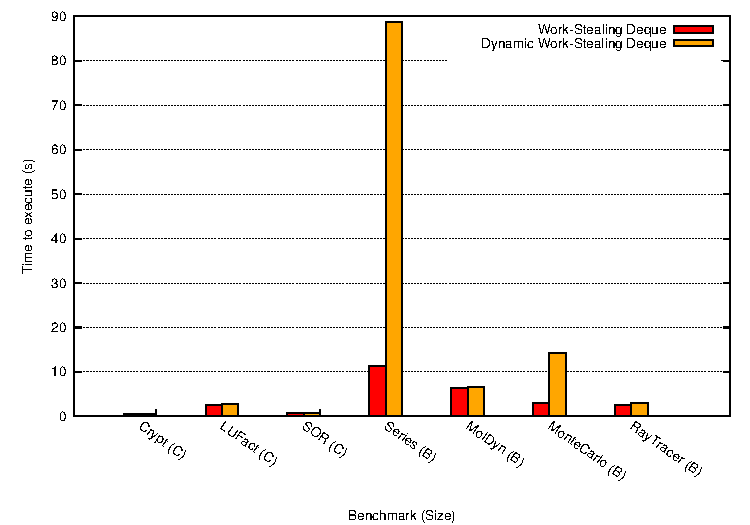
\includegraphics[width=0.5\linewidth]{queues-performance/mafushi-dynamic}
    \label{fig:queues-performance-mafushi-dynamic}
  }
  \caption{Dynamic benchmarks running on Intel Core2 Duo (Appendix
    \ref{sec:experimental-setup-marvin}) and Intel Nehalem (Appendix
    \ref{sec:experimental-setup-mafushi})}
  \label{fig:queues-performance-dynamic}
\end{figure}

\subsection{Idempotent Work-Stealing Queues}
\label{sec:performance-alternative-idempotent}

When experimenting with idempotent queues, we also implemented the
\emph{Idempotent Work-Stealing FIFO Queue} and \emph{Idempotent
  Work-Stealing LIFO Queue} to compare them to the \emph{Idempotent
  Work-Stealing Deque}. It turned out that the \emph{Idempotent
  Work-Stealing Deque} has the best performance in combination with
the intervals scheduler.

The \emph{Idempotent Work-Stealing FIFO Queue} behaves like a normal
queue: \lstinline!put()! puts tasks at the tail, and
\lstinline!take()!  and \lstinline!steal()! remove tasks at the
head. As \lstinline!take()! and \lstinline!steal()! work on the same
side of the queue, this increases contention. This

LIFO Queue $\rightarrow$ Stack! All operations work on the tail
$\rightarrow$ too much contention.

\begin{figure}[!htb]
  \centering
  \subfloat[Intel Core2 Duo: 2 threads, 2 workers]{
    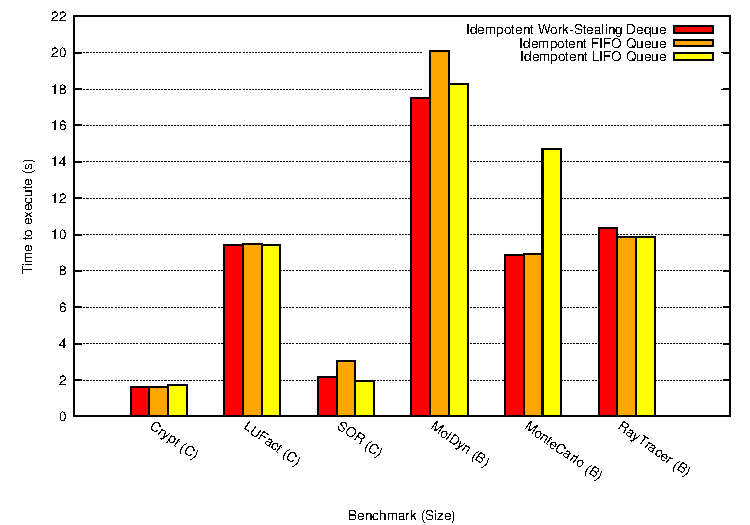
\includegraphics[width=0.5\linewidth]{queues-performance/marvin-idempotent}
    \label{fig:queues-performance-marvin-idempotent}
  }
  \subfloat[Intel Nehalem: 8 threads, 8 workers]{
    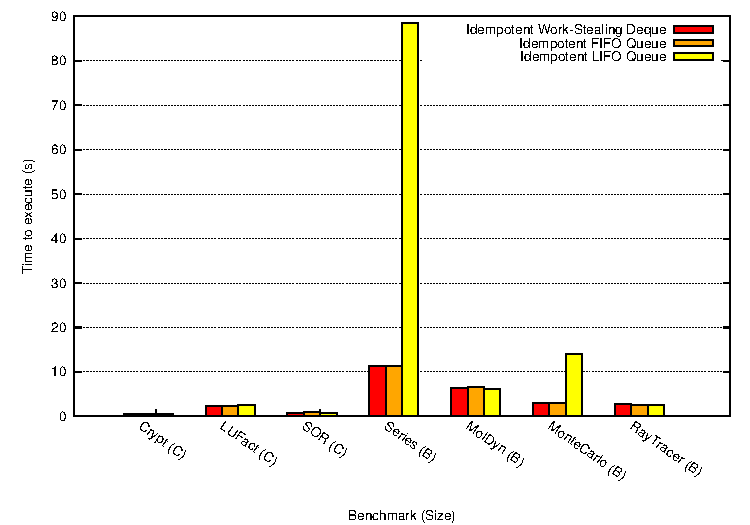
\includegraphics[width=0.5\linewidth]{queues-performance/mafushi-idempotent}
    \label{fig:queues-performance-mafushi-idempotent}
  }
  \caption{Idempotent benchmarks running on Intel Core2 Duo (Appendix
    \ref{sec:experimental-setup-marvin}) and Intel Nehalem (Appendix
    \ref{sec:experimental-setup-mafushi})}
  \label{fig:queues-performance-idempotent}
\end{figure}

\subsection{Duplicating Work-Stealing Queue}
\label{sec:performance-alternative-duplicating}

We implemented the \emph{Duplicating Work-Stealing Queue} (Section
\ref{sec:queues-alternative-implementations-duplicating-queue}) as an
alternative to the \emph{Idempotent Work-Stealing Deque}. Both use
idempotent intervals, but whereas the idempotent work-stealing deque
relies on atomic Compare-and-Swap operations and uses a tag to prevent
the ABA problem, the duplicating work-stealing queue uses a lock on
all but the critical paths. Despite the usage of locks in the
duplicating work-stealing queue we could not find any significant
performance difference to the idempotent work-stealing deque (Figure
\ref{fig:queues-performance-duplicating}).

\begin{figure}[!htb]
  \centering
  \subfloat[Intel Core2 Duo: 2 threads, 2 workers]{
    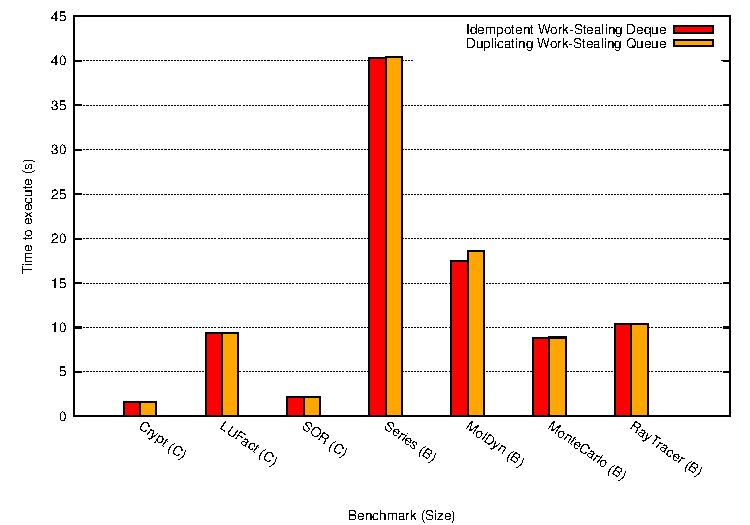
\includegraphics[width=0.5\linewidth]{queues-performance/marvin-duplicating}
    \label{fig:queues-performance-marvin-duplicating}
  }
  \subfloat[Intel Nehalem: 8 threads, 8 workers]{
    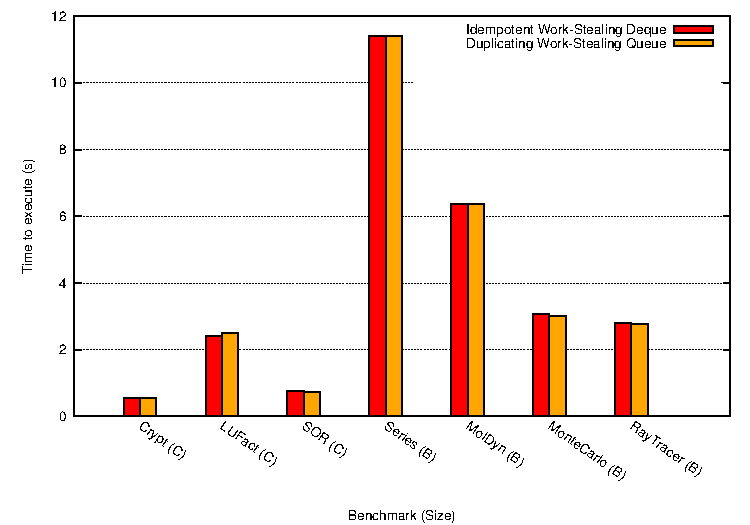
\includegraphics[width=0.5\linewidth]{queues-performance/mafushi-duplicating}
    \label{fig:queues-performance-mafushi-duplicating}
  }
  \caption{Duplicating benchmarks running on Intel Core2 Duo (Appendix
    \ref{sec:experimental-setup-marvin}) and Intel Nehalem (Appendix
    \ref{sec:experimental-setup-mafushi})}
  \label{fig:queues-performance-duplicating}
\end{figure}

\todo{Finish section ``Alternative Work-Stealing Queues''}


\section{Shared Work Queue}
\label{sec:queues-performance-shared-queue}

None of the queues we developed significantly improves work-stealing
performance on the machines we had to test them with.

$\Rightarrow\mbox{ }\le 8$ cores, mention \cite{Saha2007}.

The original work-stealing algorithm uses non-blocking algorithms to
implement queue operations \cite{Arora2001}. However, we have decided
to simplify our scheduler implementation by protecting each run queue
with its own lock. We believed that this would not impact scalability
on our machine, because others \cite{Saha2007} have reported that even
a single, centralized queue protected by a single, central lock does
not hurt performance on up to 8 CPUs, which is a decidedly worse
situation for scalability as the number of CPUs grows. Since we use
locks to protect the run queues, and our networks are static, our
implementation does not benefit from the first two advantages of
accessing the run queues at different ends. Nevertheless, this helps
with increasing locality: since the arrival of a message unblocks a
proces, placing it at the front of the ready queue increases
probability that the required data will remain in the CPU's caches.

\begin{figure}[htb]
  \centering
  \subfloat[Intel Core2 Duo: 2 threads, 2 workers]{
    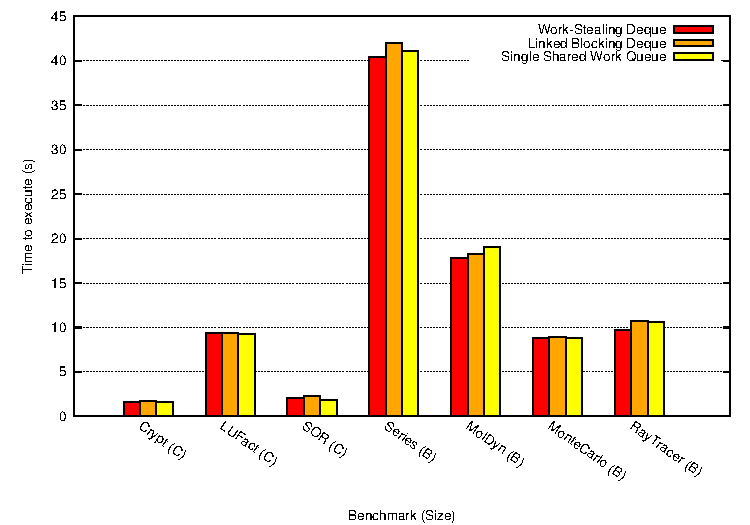
\includegraphics[width=0.5\linewidth]{queues-performance/marvin-shared-queue}
    \label{fig:queues-performance-marvin-shared-queue}
  }
  \subfloat[Intel Nehalem: 8 threads, 8 workers]{
    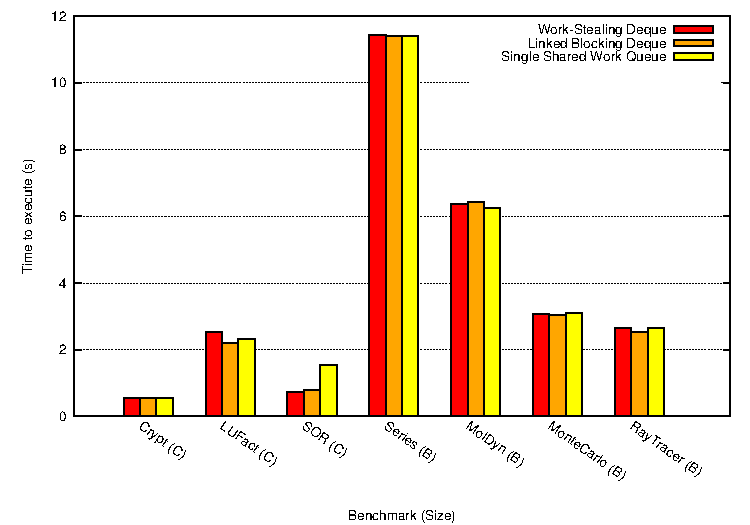
\includegraphics[width=0.5\linewidth]{queues-performance/mafushi-shared-queue}
    \label{fig:queues-performance-mafushi-shared-queue}
  }
  \caption{Shared-Queue benchmarks running on Intel Core2 Duo (Appendix
    \ref{sec:experimental-setup-marvin}) and Intel Nehalem (Appendix
    \ref{sec:experimental-setup-mafushi})}
  \label{fig:queues-performance-shared-queue}
\end{figure}

Conclusion: To really study the impact of work-stealing queues on the
intervals implementation we need to do extend our experiments on
machines with more than 8 cores.

\todo{Finish section ``Shared Work Queue''}
\todo{Finish chapter ``Performance''}


%%% Local Variables: 
%%% mode: latex
%%% TeX-master: "thesis"
%%% End: 
